\documentclass{article}

% if you need to pass options to natbib, use, e.g.:
\PassOptionsToPackage{numbers, compress}{natbib}
% before loading nips_2017
%
% to avoid loading the natbib package, add option nonatbib:
% \usepackage[nonatbib]{nips_2017}

%\usepackage{nips_2017}
\usepackage[final]{nips_2017}
\bibliographystyle{abbrvnat}

% to compile a camera-ready version, add the [final] option, e.g.:
%\usepackage[final]{nips_2017}

\usepackage[utf8]{inputenc} % allow utf-8 input
\usepackage[T1]{fontenc}    % use 8-bit T1 fonts
\usepackage{hyperref}       % hyperlinks
\usepackage{url}            % simple URL typesetting
\usepackage{booktabs}       % professional-quality tables
\usepackage{amsfonts}       % blackboard math symbols
\usepackage{nicefrac}       % compact symbols for 1/2, etc.
\usepackage{microtype}      % microtypography
\usepackage{amsmath}
\usepackage{algorithm}
\usepackage{algpseudocode}
\usepackage{graphicx}
\usepackage{todonotes}
\usepackage{xargs}
\usepackage{booktabs}

\providecommand{\scan}{\text{SCAN}}
\providecommand{\reduce}{\text{REDUCE}}
% declaration of the new block
\algblock{ParFor}{EndParFor}
% customising the new block
\algnewcommand\algorithmicparfor{\textbf{parfor}}
\algnewcommand\algorithmicpardo{\textbf{do}}
\algnewcommand\algorithmicendparfor{\textbf{end\ parfor}}
\algrenewtext{ParFor}[1]{\algorithmicparfor\ #1\ \algorithmicpardo}
\algrenewtext{EndParFor}{\algorithmicendparfor}

\newcommandx{\Chris}[2][1=]{\todo[linecolor=red,backgroundcolor=red!25,bordercolor=red,#1]{#2}}
\newcommandx{\Eric}[2][1=]{\todo[linecolor=blue,backgroundcolor=blue!25,bordercolor=blue,#1]{#2}}
\newcommandx{\thiswillnotshow}[2][1=]{\todo[disable,#1]{#2}}

\title{Parallelizing Linear Recurrent Neural Nets Over Sequence Length}

% The \author macro works with any number of authors. There are two
% commands used to separate the names and addresses of multiple
% authors: \And and \AND.
%
% Using \And between authors leaves it to LaTeX to determine where to
% break the lines. Using \AND forces a line break at that point. So,
% if LaTeX puts 3 of 4 authors names on the first line, and the last
% on the second line, try using \AND instead of \And before the third
% author name.

\author{
  Eric Martin \\%\thanks{Use footnote for providing further
    %information about author (webpage, alternative
    %address)---\emph{not} for acknowledging funding agencies.} \\
  %Some Affiliation\\
  \texttt{eric@ericmart.in}
  %% examples of more authors
  \And
  Chris Cundy \\
  \texttt{c.cundy@berkeley.edu}
  %%\texttt{some@email.com}
  %% Affiliation \\
  %% Address \\
  %% \texttt{email} \\
  %% \AND
  %% Coauthor \\
  %% Affiliation \\
  %% Address \\
  %% \texttt{email} \\
  %% \And
  %% Coauthor \\
  %% Affiliation \\
  %% Address \\
  %% \texttt{email} \\
  %% \And
  %% Coauthor \\
  %% Affiliation \\
  %% Address \\
  %% \texttt{email} \\
}

\begin{document}
% \nipsfinalcopy is no longer used

\maketitle

\begin{abstract}
Recurrent neural networks (RNNs) are widely used to model sequential data but
their non-linear dependencies between sequence elements prevent parallelizing
training over sequence length. We show the training of RNNs with only linear
sequential dependencies can be parallelized over the sequence length using the
parallel scan algorithm, leading to rapid training on long sequences with small
minibatch size.\Chris{Thought: we could rephrase this as allowing us to break
the necessity of using large batches to train fast} We develop a
parallel linear recurrence CUDA kernel and show that it can be applied to
immediately speed up several RNN architectures by up to a factor of 9. We abstract
recent work on linear RNNs into a new framework of linear surrogate RNNs and develop
a linear surrogate for the long short-term memory unit, the GILR-LSTM, which is
able to achieve throughput 30 times greater than the currently fastest-available LSTM
implementation. We show that the GILR-LSTM is able to perform well on real-world
problems, 
\end{abstract}

\section{Introduction}
Recurrent neural networks (RNNs) are widely used for sequence modelling tasks in
domains such as natural language processing \cite{sutskever2014sequence}, speech
recognition \cite{amodei2015deep}, and reinforcement learning
\cite{hausknecht2015deep}. Most RNNs, including popular variants such as long
short-term memories (LSTMs) \cite{hochreiter1997long} and gated recurrent units
(GRUs) \cite{cho2014learning}, contain a non-linear dependency between
sequential inputs. These non-linear dependencies create a very flexible class of
models but limit the feasibility of training RNNs on long sequences as each
sequence element must be processed sequentially.  Modelling sequences of
thousands to millions of elements is important to domains such as robotics,
remote sensing, control systems, speech recognition, medicine, and finance.

The RNN serial evaluation inefficiency problem is usually mitigated by
parallelizing the forward and backward pass over a minibatch of inputs. Without
minibatches, RNN evaluation is a sequence of matrix-vector
multiplications. Minibatches transform RNN computation into a sequence of more
efficient matrix-matrix multiplications, but this speed-up brings several
disadvantages.  RNN model size is often limited by GPU memory size, and running
a forward and backward pass on a minibatch requires memory linear in the
minibatch size.  Grouping data into minibatches increases the latency of each
pass and reduces the rate of optimization steps. Finally, training with larger
minibatches damages generalization ability \cite{keskar2017large}. It is clearly
important to investigate if it is possible to parallelise RNN training without
introducing minibatches. Persistent RNNs \cite{diamos2016persistent} use a novel
implementation that can achieve high GPU utilization with very small minibatch
sizes when the recurrent state is larger than 500 elements, but even persistent
RNNs become limited by the serial evaluation inefficiency at smaller hidden
sizes.

Numerous prior works have shown strong performance from neural sequential models
with only linear dependence on earlier sequence
elements. \citet{balduzzi2016strongly} investigated RNNs with only elementwise
linear recurrence relations $h_t = \alpha_t \odot h_{t-1} + (1-\alpha_t) \odot
x_t$ and developed linear variants of LSTM and GRU that perform similarly to
standard non-linear RNNs on text generation tasks. \citet{bradbury2017quasi},
\citet{kalchbrenner2016neural}, \citet{gehring2017convolutional}, and
\citet{van2016wavenet} have successfully applied networks of convolutions over
sequences for tasks such as machine translation, language modelling, and audio
generation.  These works have observed up to an order of magnitude increase in
training throughput compared to RNN alternatives. Convolutional sequence models
typically rely on either an attention mechanism or a (possibly linear) recurrent
layer to integrate information at scales larger than the filter
width. Introduction of a recurrent layer prevents full parallelization over the
sequence length while attention mechanisms are expensive to apply on long
sequences in online inference use cases.  One dimensional convolution can be
viewed as a learnable linear finite impulse response (FIR) filter with a
parallel evaluation algorithm, while linear recurrence is a learnable linear
infinite impulse response (IIR).\Chris{Seems like an aside - take out?}

  This work parallelizes evaluation of linear recurrences through application of
the parallel scan algorithm.

Scans and reductions are computations involving repeated application of a binary
operator $\oplus$ over an array of data. Computing the sum or maximum
of an array is an example of a reduction, while a cumulative sum is a common
example of a scan operation. Throughout this work, the scan of $\oplus$ with
initial value $b$ is defined as
\begin{align*}
\scan(\oplus, [a_1, a_2, ..., a_n], b) = [(a_1 \oplus b), (a_2 \oplus a_1 \oplus b), ..., (a_n \oplus a_{n-1} ... \oplus a_1 \oplus b)]
\end{align*}
The reduction of $\oplus$ over array $A$ and initial value $b$ is denoted 
$\reduce(\oplus, A, b)$ and is the final element of $\scan(\oplus, A, b)$.
Despite their dependent computation graph, algorithms exist to parallelize scans 
and reductions when $\oplus$ is associative \cite{ladner1980parallel}.

\citet{blelloch1990prefix} shows that first order recurrences of the form
$h_t = (\Lambda_t \otimes h_{t-1}) \oplus x_t$ can be parallelized with
the parallel scan algorithm if three conditions are met:

\begin{enumerate}
\item $\oplus$ is associative: $(a \oplus b) \oplus c = a \oplus (b \oplus c)$
\item $\otimes$ is semiassociative: there exists a binary associative operator
$\odot$ such that $a \otimes (b \otimes c) = (a \odot b) \otimes c$
\item $\otimes$ distributes over $\oplus$: $a\otimes(b\oplus c) = (a\otimes b) \oplus (a \otimes c)$ 
\end{enumerate}

Considering the familiar operations in linear algebra, we see that the
associative operation of vector addition
($\boldsymbol{x} \oplus \boldsymbol{y} = \boldsymbol{x} + \boldsymbol{y}$), the
semiassociative operation of matrix-vector multiplication
($A \otimes \boldsymbol{x} = A\boldsymbol{x}$) and the associative operation of
matrix-matrix multiplication ($A \odot B=AB$) satisfy Blelloch's three
conditions, allowing $h_t = \Lambda_t h_{t-1} + x_t$ to be evaluated in parallel
over time steps \(t\) for vectors $x_t$ and square matrices $\Lambda_t$.

We investigate this idea further and deliver the following contributions:
\begin{itemize}
\item{We classify the RNNs which satisfy the conditions above, and
    show that many of the RNNs used in practice such as the Quasi-RNN are
    contained in this class}
\item{We provide an implementation of the parallel linear recurrence
    algorithm as a CUDA kernel, and show that it speeds up training of
    the SRU and QRNN architectures by factors of up to 9x}
\item{We describe how several recent linear RNNs can be described as
    linear surrogates for nonlinear architectures. We introduce a linear
    surrogate for the LSTM and show that we are able to train it
    with a speedup of 5-10x compared to the CuDNN-LSTM when we use the
    parallel linear recurrence algorithm.}
\end{itemize}

\section{Parallel linear recurrence}
As the method is
essential to this work, Algorithm 1 presents the parallel linear recurrence
algorithm for the interested reader.
\begin{algorithm}
  \label{alg:plr}
\caption{Parallel linear recurrence on $p$ processors}
\begin{algorithmic}[1]
  \State Let $y = [(\Lambda_1, x_1), (\Lambda_2, x_2), ..., (\Lambda_T, x_T)]$
  \State Let binary operator $\bullet$ act as $(\Lambda, x) \bullet h = \Lambda h + x$
  \State Let $S_0=1, S_i < E_i, E_i + 1 = S_{i+1}, E_{p-1}=T$ for $i$ in $0,p-1$

  \\
  \ParFor{$i \gets 0,p-1$}
    \State $P_i = \reduce(\odot, \Lambda_{S_i:E_i}, I)$
    \State $R_i = \reduce(\bullet, y_{S_i:E_i}, 0)$
  \EndParFor

  \\
  \State Let $z = [(P_0, R_0), (P_1, R_1), ..., (P_p, R_p)]$.
  \State $C = \scan(\bullet, z, h_0)$   \Comment{compute $C_i = P_i C_{i-1} + R_i$ with $C_{-1}=h_0$}

  \\
  \ParFor{$i \gets 0,p-1$}
    \State $h_{S_i:E_i} = \scan(\bullet, y_{S_i:E_i}, C_{i-1})$
  \EndParFor
  
  \State \Return $h$
\end{algorithmic}
\end{algorithm}

\subsection{Theoretical performance}
The cost of a serial scan over a sequence of length $T$ is 
$C_\text{sscan} \in \mathcal{O}((C_\otimes + C_\oplus)T)$, compared to the parallel scan cost
$C_\text{pscan} \in \mathcal{O}(2(C_\odot + C_\otimes + C_\oplus)(T/p + \lg p))$ \cite{blelloch1990prefix},
where \(p\) is the number of available parallel cores. 
If $h_t$ is a vector of dimension $n$ then 
$C_\odot \in  \mathcal{O}(n^3), C_\otimes \in \mathcal{O}(n^2), C_\oplus \in \mathcal{O}(n)$ giving
$C_\text{pscan} \in \mathcal{O}(2(n^3 + n^2 + n)(T/p + \lg p))$ and 
$C_\text{sscan} \in \mathcal{O}((n^2 + n)T)$. The $\mathcal{O}(n^3)$ cost of the matrix
multiplication in the parallel algorithm can counter-act any parallel speedups for
sufficiently large hidden states and lead to a slower algorithm overall.

To avoid this problem, we will only consider diagonal matrices $\Lambda_t$, in
which case both matrix-matrix and matrix-vector multiplication have cost
proportional to $n$ and $C_\text{pscan}\in \mathcal{O}(6n(T/p + \lg p))$ and
$C_\text{sscan} \in \mathcal{O}(2nT)$. Assuming $p \ll T$, then $C_\text{pscan} \le
C_\text{sscan}$ when $p \ge 3$.\Chris{Can include the actual speedup
  factor, \(\alpha = \frac{PT}{3(T + \lg(p))}\).}
As we are only considering diagonal matrices,
we write the linear recurrence as $h_t = \lambda_t \odot h_{t-1} + x_t$
where $\odot$ indicates elementwise multiplication.

Limiting $\Lambda_t$ to be diagonal may seem like a severe constraint but there are
several reasons to do so beyond the unfavorable parallelization performance. Relatively few neural
network models use separate recurrent matrices for each sequence element and using these
separate matrices would require potentially prohibitive $n^2T$ memory.\Chris{I can't
seem to find anyone explicitly saying this before from a quick google.}
Applying
the same matrix $\Lambda$ to each sequence element is also unappealing considering that a matrix
multiplication can be thought of as a rotation and a scaling. The same rotation at every
element seems unlikely to be useful, and the scaling is exactly what's captured in diagonal
vectors $\lambda_t$. Recurrent coefficient vectors $\lambda_t$ provide enough flexibility
to implement schemes such as exponential moving averages or a gating mechanism.


\subsection{Backpropagation}
\begin{align*}
\nabla_{h_T}L &= \frac{\partial L}{\partial h_T} \\
\nabla_{h_t}L &= \frac{\partial h_{t+1}}{\partial h_t} \odot \nabla_{h_{t+1}} L + \frac{\partial L}{\partial h_t} \\ 
&= \lambda_{t+1} \odot \nabla_{h_{t+1}} L + \frac{\partial L}{\partial h_t} \\
\nabla_{\lambda_t}L &= \frac{\partial h_t}{\partial\lambda_t} \odot \nabla_{h_t}L = h_{t-1} \odot \nabla_{h_t}L \\
\nabla_{x_t}L &= \nabla_{h_t} L \\
\nabla_{h_0}L &=  \frac{\partial h_1}{\partial h_0} \odot \nabla_{h_1} L = \lambda_1 \odot \nabla_{h_1} L
\end{align*}

The backpropagation equations center around a linear recurrence over $\frac{\partial L}{\partial h_t}$ in the reverse order of the original sequence. This allows for parallelizing both the forwards and backwards pass of a linear RNN over the sequence length.

\subsection{Implementation}
In 2017, GPUs commonly used in deep learning consist of between 640 and 3200
concurrently executing warps. Each warp operates on 32 single precision floating
point numbers in parallel.

This work implemented parallel linear recurrence as a CUDA kernel with bindings
into the TensorFlow \cite{abadi2016tensorflow} framework. Each warp acts as a
processor, which means the algorithmic parallelizability $p$ is up to 3200 and the theoretical
parallelization speedup factor is up to several hundred.  The 32 lanes of each
warp work on different elements of the recurrence vector in parallel. These
implementation details mean that peak performance is only obtained on sequences
of at least several thousand steps on at least a 32 element vector.

\section{Models}
Parallel linear recurrence can be used to construct a wide variety of differentiable modules that can be evaluated in parallel. Common applications of linear recurrence include gating schemes and exponential moving averages. Although linear recurrence values can depend only linearly on previous elements, the stacking of linear recurrent layers separated by non-linearities allows for a non-linear dependence on the past. In this sense the non-linear depth of a linear recurrent network is the number of layers and not the sequence length. 

\subsection{Gated impulse linear recurrent layer}
A gated impulse linear recurrent (GILR) layer transforms its $m$ dimensional inputs $x_t$ into a sequence of $n$ dimensional hidden states $h_t$:
\begin{align*}
g_t &= \sigma(Ux_t + b_g) \\
i_t &= \tau(Vx_t + b_z) \\
h_t &= g_t \odot h_{t-1} + (1-g_t)\odot i_t
\end{align*}
A GILR layer applies the same non-linear transform to each sequence element and
then accumulates the sequence elements with a non-linear gating mechanism. Gate
$g_t$ uses the sigmoid activation function to give values in [0,1] for
reasonable gating semantics, while impulse $i_t$ can use any activation function
$\tau$. Stacking GILR layers allows for rich non-linear dependence on previous
events while still taking advantage of fast parallel sequence evaluation.

\subsubsection{Impact on effective "batch size"}
Consider evaluating an RNN with recurrence $h_t = \sigma(Uh_{t-1} + Vx_t + b)$,
from $m$ inputs to $n$ hidden units on a sequence of length $T$ with minibatch
size $b$ using a serial evaluation strategy. At each of $T$ iterations, the
naive approach performs two $(b, m) \times (m, n)$ matrix
multiplications. Larger matrix multiplications achieve higher throughput due to
less IO overhead, so the better approach computes $Vx_t$ for all $t$ ahead of
time in a single $(bT, m) \times (m, n)$ matrix multiply. The non-linear
recurrence forces even the better approach to perform $T$ potentially small $(b,
m) \times (m, n)$ matrix multiplications in serial which makes performance
heavily dependent on minibatch size.

Now consider the GILR, noting that it has the same two matrix-vector
multiplications per iteration as the above RNN. The intermediate variables $g$
and $i$ can be evaluated for all $t$ with a single $(bT, m) \times (m, n)$
matrix multiplication each. Given $g$ and $i$, $h$ can be computed using a
parallel linear recurrence over $T$ vectors each of $bn$ elements. Rather than
$T$ small operations, the GILR can be evaluated over all sequence elements with
two large matrix multiplications and a parallel linear recurrence. GILR performance
is much less dependent on batch size as the matrix multiplies see an "effective
batch size" of $bT$ and $T$ is typically large.

\subsection{Linear surrogate RNNs}
\label{sec:ls-rnns}
RNNs learn a transition function $s_t = f(s_{t-1}, x_t)$ which combines previous
state $s_{t-1}$ with input $x_t$ to compute current state $s_t$. Non-linear $f$
prevents application of the parallel linear recurrence algorithm and forces slow
serial evaluation. To work around this inefficiency, note that $s_t$ serves a
dual purpose. In $s_t = f(s_{t-1}, x_t)$, $s_{t-1}$ serves as an input to $f$
summarizing the previous inputs while $s_t$ serves as the output of $f$ to be
passed to other layers of the network. We can decouple these uses and introduce
independent variables for each purpose: \(s_t\) is passed onto other layers of the network
and we introduce the linear surrogate \(\tilde{s}_t\) which is passed onto the
next state, with \(s_t = f(\tilde{s}_{t-1}, x_t)\). We are still able to choose a 
nonlinear \(f\), our only limitation being that \(\tilde{s}_t\) must be linearly
computable.  We refer to this class of model as a linear surrogate RNN
(LS-RNN). Quasi-RNNs \cite{bradbury2017quasi} are LS-RNNs using $\tilde{h}_{t-1}
= W_k x_{t-k} + ... W_1 x_{t-1}$ and strongly typed
RNNs\cite{balduzzi2016strongly} are LS-RNNs with $\tilde{h}_t=x_{t-1}$. Although
not a rule, LS-RNNs can often be parallelized over sequence length with either
convolution or linear recurrence.

As an example LS-RNN, consider an LSTM:
\begin{align*} f_t, i_t, o_t &= \sigma(U_{f,i,o} h_{t-1} + V_{f,i,o} x_t +
b_{f,i,o}) \\ z_t &= \tau(U_z h_{t-1} + V_z x_t + b_z) \\ c_t &= f_t \odot
c_{t-1} + i_t \odot z_t \\ h_t &= o_t \odot c_t
\end{align*} An LSTM has state $s_t = (h_t, c_t)$. Since $c_t$ depends only
linearly on $c_{t-1}$, no surrogate is needed for $c_t$. $h_t$ has a non-linear
dependence on $h_{t-1}$, so $h_t$ needs a linear surrogate. Introducing a GILR layer as
the surrogate, we obtain the GILR-LSTM:
\begin{align*} f_t, i_t, o_t &= \sigma(U_{f,i,o} \tilde{h}_{t-1} + V_{f,i,o} x_t
+ b_{f,i,o}) \\ z_t &= \tau(U_z \tilde{h}_{t-1} + V_z x_t + b_z) \\ c_t &= f_t
\odot c_{t-1} + i_t \odot z_t \\ h_t &= o_t \odot c_t \\ g_t &= \sigma(V_g x_t +
b_g) \\ \tilde{h}_t &= g_t \odot \tilde{h}_{t-1} + (1-g_t)\odot \tau(Wx_t + b_h)
\end{align*}

For $m$ inputs and hidden size $n$, the GILR-LSTM contains $2n(n+m)$ more
parameters than the equivalently sized LSTM to handle the mapping from $x$ to
$\tilde{h}$. More generally, a LS-RNN contains all of the same parameters as the
underlying RNN as well as some additional parameters to compute the linear
surrogate.

\section{Experiments}
We perform several experiments, first confirming that our implementation of the
parallel linear recurrence algorithm is able to achieve higher throughput than a
similarly implemented serial version of the algorithm. We show that the plr kernel
is up to 40 times faster than the serial equivalent for long sequence lengths, and
that this speedup translates to implementations of LS-RNNs such as the QRNN (where
we can get a speedup of up to 9 times).

In order to illustrate that the linearisation does not necessarily come at the
cost of expressibility, we show that the GILR-LSTM architecture, trained with
the PLR algorithm, is able to outperform the optimized CuDNN LSTM implementation
on a pathological example from the original LSTM paper
\cite{hochreiter1997long}. Finally we show that our GILR-LSTM is able to
quickly achieve state of the art results on an existing medical data
set. \Chris{I hope so\ldots}

\subsection{Throughput Benchmarks}
We first illustrate the throughput advantage of the parallel scan algorithm for
evaluating the linear recurrence. For a minibatch comprised of \(b\) sequences
of length \(T\), we define the number of events as \(bT\) and the throughput as
the number of events per second. We implement two CUDA kernels, one which
evaluates the parallel linear recurrence described in algorithm \ref{alg:plr},
and one which evaluates the linear recurrence using the straightforward serial
approach. This comparison is performed directly at the kernel level, avoiding
any overhead due to calling Tensorflow. We find that at long sequence lengths,
the PLR kernel has a distinct advantage, as shown in table
\ref{table:kernel-throughput}, with a speedup factor of 40. At short sequence
lengths, the parallel kernel does not perform well due to the extra overhead
involved in marshalling the parallel algorithm. \Chris{Important:
  What's the batch size here? Is it just one sequence? Need to say that}
\begin{table}[]
  \centering
\caption{Speedup of the PLR kernel compared to the SLR kernel, without any
  overhead from Tensorflow, for various sequence lengths and input size \(m\).}      
\label{table:kernel-throughput}
\begin{tabular}{@{}llll@{}}
Sequence Length & \(m=4\)  & \(m=32\) & \(m=128\) \\ \midrule
16              & 0.06 & 0.06 & 0.05  \\
256             & 0.22 & 0.22 & 0.86  \\
4,096           & 1.02 & 2.94 & 3.36  \\
65,536          & 38.5 & 41.8 & 17.5  \\ \bottomrule
\end{tabular}
\end{table}
  
Many of the RNNs that have been recently introduced can be implemented with a
parallel linear recurrence. Table \ref{table:rnn-throughput} shows the
throughput advantage by using a parallel linear recurrence when compared to a
serial linear recurrence. Since PLR and SLR are simply different methods for
computing the recurrence, there is no penalty incurred for this speedup - we
obtain exactly the same output.

Typically experiments will aim to maximize the memory
utilisation of the GPU, so we simulate this by choosing the product of the batch
size and the sequence length to be constant. We see that the architectures which
have fewer terms (for which the linear recurrence is a higher proportion of the
computational burden) are more effected by the switch to PLR.  This is
particularly clear in the case of the QRNN, where including a wider
convolutional window results in less time spent on the recurrence and less to
gain from the parallelization.
\begin{figure}
\begin{center}
  \begin{tabular}{@{}lrrrr@{}}
    \label{table:rnn-throughput}
Sequence Length & GILR-LSTM & SRU & QRNN(2) & QRNN(10)\\ \midrule
16 & 0.61 & 0.28 & 0.38 & 0.78\\
256 & 0.91 & 0.84 & 0.86 & 0.99\\
4,096 & 0.98 & 1.38 & 1.18 & 1.05\\
65,536 & 1.41 & 9.21 & 6.68 & 2.05\\ \bottomrule
  \end{tabular}  
\end{center}
\caption{Speedup obtained when using parallel linear recurrence compared to
  serial linear recurrence. We analyse this for several recent architectures:
  the Simple Recurrent Unit from \cite{lei2017}, the Quasi-RNN from
  \cite{bradbury2017quasi}, with a convolutional filter of size 2 and 10, and
  the GILR-LSTM which we introduce in section \ref{sec:ls-rnns}. To give a fair
  model of a typical use-case maximising the memory usage of the GPU, we set
  batch size \(b\) such that \(Tb = 65536\) for a sequence length \(T\).}
\end{figure}

Finally, we compare the throughput of the linear surrogate LSTM to the current
fastest available implementation of the LSTM, the CuDNN-LSTM. Figure
\ref{fig:tp_perf} shows that our GILR-LSTM has higher throughput for most of the
low-batch-size regime, with a 30x speedup at a sequence length of 65,536. Recent
work \cite{keskar2017large} has suggested that small mini-batches may aid
generalization by encouraging the discovery of shallow minima. The GILR-LSTM
allows us to achieve high throughput for all choices of minibatch size and
sequence length.

%%%%%%%%%%%%%%%%%%%%%%%%%%%%%%%%%%%%%%%%%%%%%%%%%%%%%%%%%%%%%%%%%%%%%%%%%%%%%%%%%%%%
% The computational performance of the LSTM and GILR-LSTM models were compared       %
% across a wide range of minibatch sizes and sequence lengths. Although the 234    %
% unit GILR-LSTM has a similar number of parameters to the 256 unit LSTM, we         %
% measured the computational performance of a 256 unit GILR-LSTM to observe any      %
% impact of the linear surrogate calculation. The serial evaluation of the LSTM    %
% causes its throughput to be independent of the sequence length as a doubling of  %
% sequence length causes a doubling of runtime. Notably, the GILR-LSTM can achieve a %
% higher throughput by running on one 8192 event sequence at a time than an LSTM   %
% running with 256 sequence minibatches. Similar speedups were found for           %
% inference.                                                                       %
%%%%%%%%%%%%%%%%%%%%%%%%%%%%%%%%%%%%%%%%%%%%%%%%%%%%%%%%%%%%%%%%%%%%%%%%%%%%%%%%%%%%

Unlike the previous case, these speedups do come at a cost. The GILR-LSTM
architecture is different to the canonical LSTM, and it's possible that the loss
of model capacity outweighs the speedup in training. The following experiment
shows that the GILR-LSTM is able to outperform the LSTM on an example originally
designed to illustrate the advantages of the LSTM.

\begin{figure}[t]
\centering
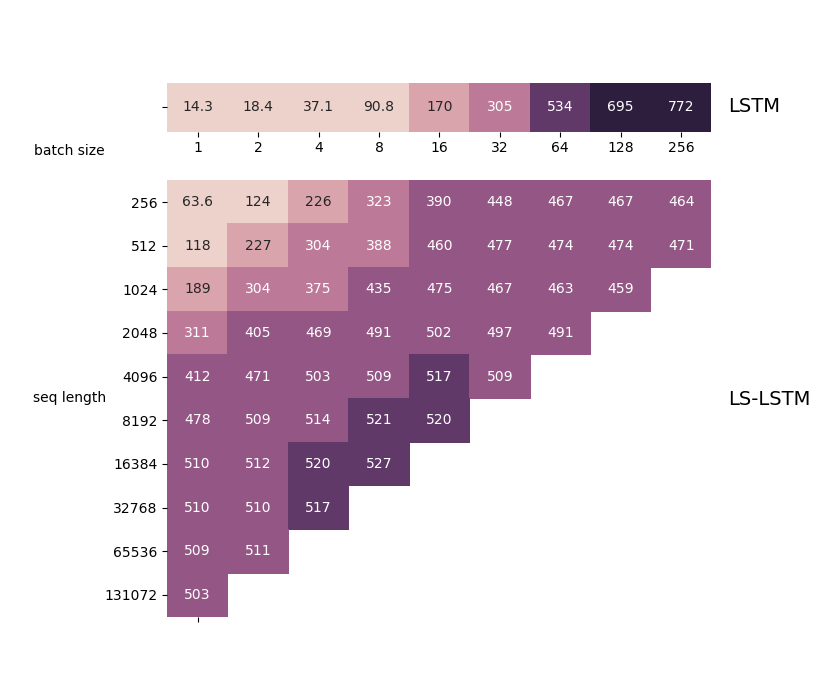
\includegraphics[width=12cm]{cudnn_heatmap.png}
\caption{Throughput comparison between LSTM-256-256 with GILR-LSTM-256-256, with a
  32-dimensional input and a 2-dimensional output, for various batch sizes and
  sequence lengths.The LSTM only has a single row of data because its throughput
  is independent of sequence length. Entries are missing from the GILR-LSTM table
  because there was not enough memory on the GPU to handle such large batch
  sizes and sequences.}
\label{fig:tp_perf}
\end{figure}


% Experiments were performed on the N-MNIST \cite{orchard2015converting} dataset. N-MNIST captures the MNIST digit dataset \cite{lecun1998mnist} by panning
% an event driven camera over each digit. Each example in N-MNIST is a sequence of single pixel events (x, y, polarity, timestamp) where
% x and y each indicate a pixel position in [0, 33], polarity indicates whether the pixel was switching on or off, and timestamp is the time of the event in microseconds. Videos produced from the event data show that positive polarity events are often located on the leading edge of the digit motion and negative polarity events on the trailing edge. Between the 60,000 digits in the training set, N-MNIST contains approximately 250 million pixel events with sequence lengths ranging from 500 to 8000 and averaging 4000 events.

% We attempt to forecast 50 events ahead in N-MNIST using a two layer LSTM with 256 units per layer and a two layer GILR-LSTM with 234 units per layer. The GILR-LSTM layer size was selected so that it had slightly fewer parameters than the LSTM. Each model transformed the incoming event position into a 40-dimensional embedding vector which was then combined with the polarity to produce a 41 dimensional input. Both models output a $2 \mathbf{x} 34^2$ matrix containing two future event location probability distributions conditioned on the polarity of the future event. The training algorithm only considers the probability distribution of the true future polarity and uses the cross entropy loss function. The Adam \cite{kingma2014adam} optimization algorithm and Glorot \cite{glorot2010understanding} initialization scheme were used. Training on a minibatch of size $b$ with sequence length $T$ consisted of uniformly sampling $b$ N-MNIST sequences and then extracting a single random $T$ element subsequence (and its 50 element ahead forecast) from the sequence. Sequences less than $T$ elements were padded out to length $T$, and there was a "burn-in" of 30 events at the start of each sequence where no predictions were made. An epoch was defined as a pass over as many pixel events as there are in the full training set.

% All experiments were performed using TensorFlow 1.0 \cite{abadi2016tensorflow} on a single Nvidia K80 GPU running for up to 18 hours. The LSTM model was computed using TensorFlow's dynamic\_rnn and BasicLSTMCell routines which are slower than but algorithmically similar to the cuDNN LSTM implementation.

% \subsection{Training performance}
% The speed of neural net training is not solely determined by the training throughput but also by the frequency of optimization steps. As an example, a batch method may process inputs at the same rate as a minibatch method, but the minibatch method will generally converge much faster on large datasets. On an infinite dataset, the batch method never takes a single optimization step regardless of its throughput. With this example in mind, it is clear that achieving fast training is a balancing act between training data throughput and optimization step latency and that training performance should be evaluated with training curves and not just throughput numbers such as time per epoch.

% The LSTM and GILR-LSTM offer differ latency and throughput tradeoffs. LSTM throughput depends only on minibatch size but LSTM latency depends on both minibatch size and sequence length. Experiments were conducted training the LSTM models with minibatch size 256 and sequence lengths 128, 256, 512, and 1024. Figure \ref{fig:learning_curves} shows the smaller sequence lengths led to faster initial learning but inferior final performance. 

% The throughput and latency of the GILR-LSTM are both influenced by batch size and sequence length. Several GILR-LSTMs were trained with batch size 16 and sequence length 1024. This combination was chosen because of the nearly maximum throughput, the low latency, and the ease of building a minibatch given the distribution of sequence lengths in the data set. The 234 unit GILR-LSTM reaches a better training loss in roughly 4.5 hours than any of the LSTMs could reach in 18 hours. This experimental evidence indicates the GILR-LSTM is as powerful of a model as the LSTM and can be trained in a fraction of the time.

% \begin{figure}[t]
% \centering
% 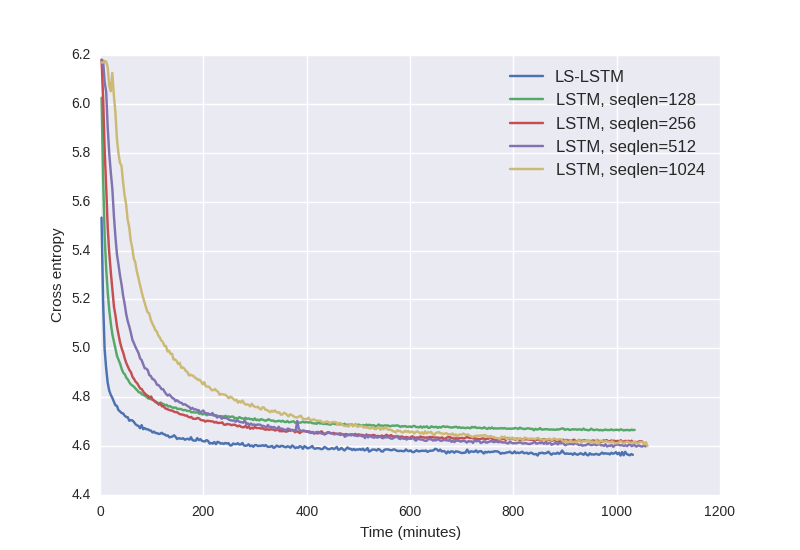
\includegraphics[width=12cm]{lc2.png}
% \caption{The LSTM models had a direct relationship between sequence length and training curve: the shorter the sequence length, the faster the initial learning and
% the higher the final loss. The faster initial learning is explained by the decreased
% latency of optimization steps and the higher final loss is explained by the
% inability to learn long dependencies. The GILR-LSTM has 234 units per hidden
% layer to have the same number of parameters as the 256 unit LSTMs.}
% \label{fig:learning_curves}
% \end{figure}

% \subsection{Test performance}
% \begin{table}[h]
%   \caption{N-MNIST test results}
%   \label{test-results}
%   \centering
%   \begin{tabular}{lllll}
%     \toprule
%     & Train Cross Entropy     & Test Cross Entropy     & Top-5 Accuracy & Top-20 Accuracy \\
%     \midrule
%     GILR-LSTM 			&  \textbf{4.567} & 4.856           & 10.51\% & 36.70\%   \\
%     LSTM, seqlen=128    & 4.664 & \textbf{4.846}  & \textbf{10.62\%} & \textbf{37.08\%}   \\
%     LSTM, seqlen=256    & 4.620                & 4.906           & 10.11\% & 35.40\%   \\
%     LSTM, seqlen=512    & 4.602                & 4.883           & 10.45\% & 36.32\%   \\
%     LSTM, seqlen=1024   & 4.611                & 4.880           & 10.32\% & 35.92\%   \\
%     \bottomrule
%   \end{tabular}
% \end{table}
% Beyond cross entropy on train and test, we also evaluated top-$k$ accuracy for $k=5, 20$. A probability distribution is top-$k$ correct if it assigns the realized location one of the
% $k$ largest probabilities. N-MNIST contains 1156 pixel positions, so top-5 and top-20 accuracy are equivalent to localizing the future to 0.43\% and 1.7\% of pixels. 

% No regularization was attempted and all of the models overfit, as indicated by the best test performance from the model with the worst train performance. Table \ref{test-results} contains the full test results. Our focus was the fast training of powerful models, and we leave regularizing parallel linear recurrences and LS-RNNs to future work. Although not tested, it is possible that the GILR-LSTM generalized better than the LSTMs trained on long sequences due to the much smaller minibatch size of GILR-LSTM leading to a wider minima.

\subsection{Synthetic Example}
In order to demonstrate how PLR may be used to speed up tasks that the LSTM is
well-suited for, we tackle a pathological inference problem. Originally
introduced as example 2b from Hochreiter and Schmidhtbuer's introduction of the
LSTM, \cite{hochreiter1997long}, it involves storing a number for a very long
sequence of time steps. We have an alphabet of size \(p\) with each character
represented as a particular one-hot vector in this space. We input a sequence of
\(n\) of these vectors, chosen at random (with replacement). The first vector in
the sequence is always the same, up to the sign of the component (i.e. it is \(\pm
\boldsymbol{p_0} \).

The two signs on the first component separate the sequences into two sets. The
whole sequence is fed into the LSTM and we aim to learn to classify the
sequences. This requires remembering the first element over the length of the
sequence. Due to the large throughput of the GILR-LSTM, we would expect that it
would do better when the sequence length is large. In the original formulation
of the problem (dealing in the regime with around one hundred timesteps)
, \(p\) is set equal to \(n\). Since this would make the size of the input data
grow impracticaly large as \(\mathcal{O}(n^2)\) for long sequences, we fix \(p =
128\) and vary \(n\).

We generated three sets of data: for \(n\) equal to 1,024, 8,192, and
1,048,576. For each of these we compared a two-layer GILR-LSTM with 512 hidden
units to a canonical LSTM network with roughly the same number of parameters. We
could imagine using a two-layer LSTM with 512 hidden units in each layer, or a
one-layer LSTM with 1024 hidden units.

Initial experiments showed that the two-layer LSTM was much quicker to converge
than the one-layer LSTM, so here we compare the GILR-LSTM to the two-layer
CudnnLSTM.  We ran all experiments on a NVIDIA K80 GPU, choosing the largest
minibatch size which fit into the GPU memory, with five runs per configuration
allowing us to find the average and standard deviation of the time and number of
iterations to convergence. For all CUDA runs, a brief search over learning rate
and batch size was carried out to find the parameters which allow the network to
converge most rapidly. The criterion for convergence was five consecutive
minibatches giving 100\% accuracy. As can be seen from the learning curves
in figure \ref{fig:synthetic_training}, this was a reasonable criterion. For the
longest sequence-length, we didn't observe the CuDNN-LSTM converging.
\begin{figure}
  \centering
  \begin{minipage}{0.5\textwidth}
    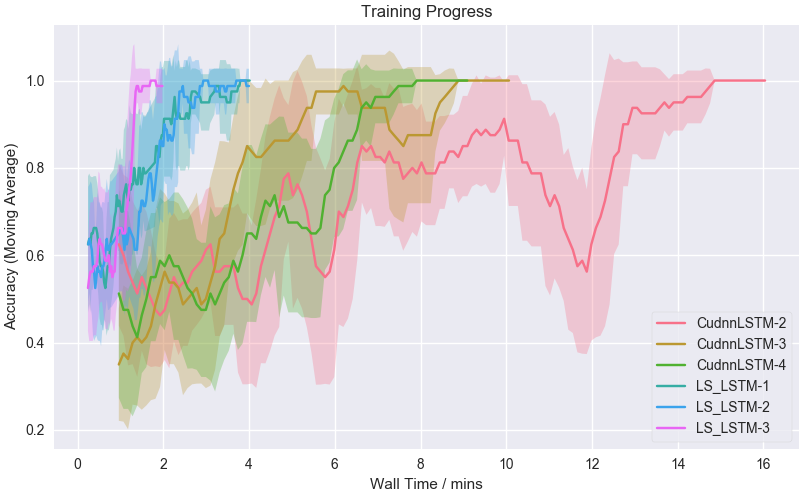
\includegraphics[width=1.0\textwidth]{./1k_synthetic.png}
  \end{minipage}%
    \begin{minipage}{0.5\textwidth}
    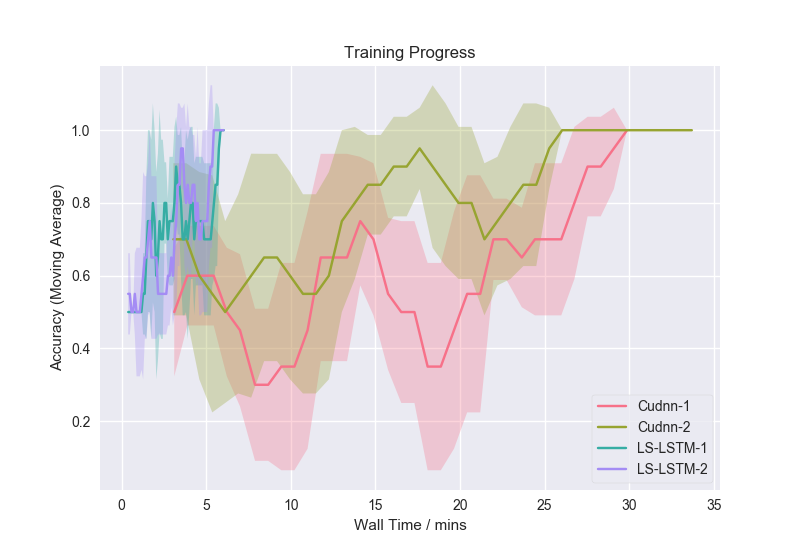
\includegraphics[width=1.0\textwidth]{./8k_synthetic.png}      
  \end{minipage}
  \begin{minipage}{0.6\textwidth}
    \includegraphics[width=1.0\textwidth]{./1M_synthetic.png}      
  \end{minipage}
  \caption{Training curves for GILR-LSTM and CUDNNLSTM architectures for various
  sequence lengths. (Clockwise from top-left: 1024, 8192, 1048576)}
    \label{fig:synthetic_training}
  \end{figure}
  
\begin{table}[]
\centering
\caption{Performance of the GILR-LSTM compared to CUDA-optimised CudnnLSTM
  implementation on problem 2b from (cite '97). We see that the GILR-LSTM has a clear
  advantage in training speed as the sequence length increases.
  We did not observe the Cudnn-LSTM converging for the longest task, even after several days.
  {\scriptsize *For the longest sequence length, the number of hidden units was decreased to
    64 for both architectures so that the net could fit in memory. }    }
\label{my-label} 
\begin{tabular}{@{}lllllll@{}} \toprule Sequence Length &
\multicolumn{2}{c}{\textbf{1,024}} & \multicolumn{2}{c}{\textbf{8,192}} &
\multicolumn{2}{c}{\textbf{1,048,576\(^*\)}} \\ \midrule &CuDNN& G &
C &GILR&CuDNN&GILR\\ \cmidrule(l){2-7} Iterations (1000s) &
                     1.0 %bs=8
                     \(\pm\) 0.4 & 0.55 %bs=8
                                    \(\pm\) 0.04 & 0.44 %bs=8
                                                   \(\pm\) 0.05 & 0.56 %bs=8
                                                                 \(\pm\) 0.16
                                                               &-& 14 \(\pm\) 3 \\
\begin{tabular}[c]{@{}l@{}}Wall Clock time (hours)\end{tabular} &
0.28 \(\pm\) 0.08 & 0.031 \(\pm\) 0.002 & 0.58 \(\pm\) 0.06 & 0.10 \(\pm\) 0.03
&-& 9.7 \(\pm\) 1.7 \\ \bottomrule
\end{tabular}
\end{table}

\subsection{Medical Example}
A common application of RNNs is in medicine. In order to illustrate the
increased performance that the plr algorithm allows, we implement an GILR-LSTM
on the problem presented in \Chris{CITE}, the 2016 PhysioNet/Computing in
Cardiology Challenge 2016.  The aim of the Classification of Normal/Abnormal
Heart Sound Recordings challenge is to determine which of a set of EEGs are
produced by people with abnormal hearts.  The data is recorded from a variety of
sources and split into a training and testing set. The testing set is not
publicly available, but can be evaluated through a web portal. The top results
cover a large range of techniques, but generally rely on featurization of the
raw EEG records. We want to see if we are able to leverage our advantage at high
sequence-lenghts to train directly on the raw EEG. The EEGs are sampled at 2,000
Hz and range in length from several seconds to more than one hundred seconds,
giving a max sequence length of over 200,000. Since the testing server is not
equipped with a GPU, we cannot run PLR in the testing step. We resample the
records to 250 Hz so that we are able to evaluate the test results in a
reasonable amount of time, padding all records that are shorter than the longest.


The training set of data is unbalanced, with 75\% of the data corresponding to
normal hearts. We rebalance the data by oversampling the abnormal data by a factor
of three, including each abnormal heart three times. 

Key points are:
\begin{itemize}
\item{With the fast training of the GILR-LSTM / PLR, we can train quickly on very
    long sequence-lengths}
\item{Allows us to get state-of-the-art results, even when performing very quickly
    and with little hyperparameter tuning}
\end{itemize}

NEED TO GET THOSE RESULTS!

  
\section{Conclusion}
Parallel linear recurrence is an extremely powerful algorithm and the GILR-LSTM is just one
of many possible models that can be built with it. Future applications of parallel linear recurrence could include sequences orders of magnitude longer than N-MNIST, the development of parallel computable differentiable memory modules, and the combination of linear recurrence with convolutional sequence models. Besides future research, existing models such as Quasi-RNNs and strongly typed RNNs that already contain linear recurrences can immediately benefit from parallel linear recurrence. This work demonstrates the GILR-LSTM significantly accelerates the training of small to medium sized LSTMs. Although similar techniques have been used before, the now explicit concept of linear surrogacy provides a framework for future development and analysis of fast sequence models.

We intend to expand upon the experiments section and open-source the parallel linear recurrence kernel in the near future.

\subsubsection*{Acknowledgments}
We would like to acknowledge Kevin Bowers, Alex Meiburg, JD Co-Reyes, Carson
McNeil, Andy Palan, and several others for fruitful conversations and guidance.

\begin{thebibliography}{19}
\providecommand{\natexlab}[1]{#1}
\providecommand{\url}[1]{\texttt{#1}}
\expandafter\ifx\csname urlstyle\endcsname\relax
  \providecommand{\doi}[1]{doi: #1}\else
  \providecommand{\doi}{doi: \begingroup \urlstyle{rm}\Url}\fi

\bibitem[Abadi et~al.(2016)Abadi, Agarwal, Barham, Brevdo, Chen, Citro,
  Corrado, Davis, Dean, Devin, et~al.]{abadi2016tensorflow}
M.~Abadi, A.~Agarwal, P.~Barham, E.~Brevdo, Z.~Chen, C.~Citro, G.~S. Corrado,
  A.~Davis, J.~Dean, M.~Devin, et~al.
\newblock Tensorflow: Large-scale machine learning on heterogeneous distributed
  systems.
\newblock \emph{arXiv preprint arXiv:1603.04467}, 2016.

\bibitem[Amodei et~al.(2015)Amodei, Anubhai, Battenberg, Case, Casper,
  Catanzaro, Chen, Chrzanowski, Coates, Diamos, et~al.]{amodei2015deep}
D.~Amodei, R.~Anubhai, E.~Battenberg, C.~Case, J.~Casper, B.~Catanzaro,
  J.~Chen, M.~Chrzanowski, A.~Coates, G.~Diamos, et~al.
\newblock Deep speech 2: End-to-end speech recognition in english and mandarin.
\newblock \emph{arXiv preprint arXiv:1512.02595}, 2015.

\bibitem[Balduzzi and Ghifary(2016)]{balduzzi2016strongly}
D.~Balduzzi and M.~Ghifary.
\newblock Strongly-typed recurrent neural networks.
\newblock In \emph{Proceedings of The 33rd International Conference on Machine
  Learning}, pages 1292--1300, 2016.

\bibitem[Blelloch(1990)]{blelloch1990prefix}
G.~E. Blelloch.
\newblock Prefix sums and their applications.
\newblock 1990.

\bibitem[Bradbury et~al.(2017)Bradbury, Merity, Xiong, and
  Socher]{bradbury2017quasi}
J.~Bradbury, S.~Merity, C.~Xiong, and R.~Socher.
\newblock Quasi-recurrent neural networks.
\newblock In \emph{International Conference on Learning Representations
  (ICLR)}, 2017.

\bibitem[Cho et~al.(2014)Cho, Van~Merri{\"e}nboer, Gulcehre, Bahdanau,
  Bougares, Schwenk, and Bengio]{cho2014learning}
K.~Cho, B.~Van~Merri{\"e}nboer, C.~Gulcehre, D.~Bahdanau, F.~Bougares,
  H.~Schwenk, and Y.~Bengio.
\newblock Learning phrase representations using rnn encoder-decoder for
  statistical machine translation.
\newblock \emph{arXiv preprint arXiv:1406.1078}, 2014.

\bibitem[Diamos et~al.(2016)Diamos, Sengupta, Catanzaro, Chrzanowski, Coates,
  Elsen, Engel, Hannun, and Satheesh]{diamos2016persistent}
G.~Diamos, S.~Sengupta, B.~Catanzaro, M.~Chrzanowski, A.~Coates, E.~Elsen,
  J.~Engel, A.~Hannun, and S.~Satheesh.
\newblock Persistent rnns: Stashing recurrent weights on-chip.
\newblock In \emph{International Conference on Machine Learning}, pages
  2024--2033, 2016.

\bibitem[Gehring et~al.(2017)Gehring, Auli, Grangier, Yarats, and
  Dauphin]{gehring2017convolutional}
J.~Gehring, M.~Auli, D.~Grangier, D.~Yarats, and Y.~N. Dauphin.
\newblock Convolutional sequence to sequence learning.
\newblock \emph{arXiv preprint arXiv:1705.03122}, 2017.

\bibitem[Glorot and Bengio(2010)]{glorot2010understanding}
X.~Glorot and Y.~Bengio.
\newblock Understanding the difficulty of training deep feedforward neural
  networks.
\newblock In \emph{Aistats}, volume~9, pages 249--256, 2010.

\bibitem[Hausknecht and Stone(2015)]{hausknecht2015deep}
M.~Hausknecht and P.~Stone.
\newblock Deep recurrent q-learning for partially observable mdps.
\newblock In \emph{2015 AAAI Fall Symposium Series}, 2015.

\bibitem[Hochreiter and Schmidhuber(1997)]{hochreiter1997long}
S.~Hochreiter and J.~Schmidhuber.
\newblock Long short-term memory.
\newblock \emph{Neural computation}, 9\penalty0 (8):\penalty0 1735--1780, 1997.

\bibitem[Kalchbrenner et~al.(2016)Kalchbrenner, Espeholt, Simonyan, Oord,
  Graves, and Kavukcuoglu]{kalchbrenner2016neural}
N.~Kalchbrenner, L.~Espeholt, K.~Simonyan, A.~v.~d. Oord, A.~Graves, and
  K.~Kavukcuoglu.
\newblock Neural machine translation in linear time.
\newblock \emph{arXiv preprint arXiv:1610.10099}, 2016.

\bibitem[Keskar et~al.(2017)Keskar, Mudigere, Nocedal, Smelyanskiy, and
  Tang]{keskar2017large}
N.~S. Keskar, D.~Mudigere, J.~Nocedal, M.~Smelyanskiy, and P.~T.~P. Tang.
\newblock On large-batch training for deep learning: Generalization gap and
  sharp minima.
\newblock 2017.

\bibitem[Kingma and Ba(2014)]{kingma2014adam}
D.~Kingma and J.~Ba.
\newblock Adam: A method for stochastic optimization.
\newblock \emph{arXiv preprint arXiv:1412.6980}, 2014.

\bibitem[Ladner and Fischer(1980)]{ladner1980parallel}
R.~E. Ladner and M.~J. Fischer.
\newblock Parallel prefix computation.
\newblock \emph{Journal of the ACM (JACM)}, 27\penalty0 (4):\penalty0 831--838,
  1980.

\bibitem[LeCun et~al.(1998)LeCun, Cortes, and Burges]{lecun1998mnist}
Y.~LeCun, C.~Cortes, and C.~J. Burges.
\newblock The mnist database of handwritten digits, 1998.

\bibitem[Orchard et~al.(2015)Orchard, Jayawant, Cohen, and
  Thakor]{orchard2015converting}
G.~Orchard, A.~Jayawant, G.~Cohen, and N.~Thakor.
\newblock Converting static image datasets to spiking neuromorphic datasets
  using saccades.
\newblock \emph{arXiv preprint arXiv:1507.07629}, 2015.

\bibitem[Sutskever et~al.(2014)Sutskever, Vinyals, and
  Le]{sutskever2014sequence}
I.~Sutskever, O.~Vinyals, and Q.~V. Le.
\newblock Sequence to sequence learning with neural networks.
\newblock In \emph{Advances in neural information processing systems}, pages
  3104--3112, 2014.

\bibitem[van~den Oord et~al.(2016)van~den Oord, Dieleman, Zen, Simonyan,
  Vinyals, Graves, Kalchbrenner, Senior, and Kavukcuoglu]{van2016wavenet}
A.~van~den Oord, S.~Dieleman, H.~Zen, K.~Simonyan, O.~Vinyals, A.~Graves,
  N.~Kalchbrenner, A.~Senior, and K.~Kavukcuoglu.
\newblock Wavenet: A generative model for raw audio.
\newblock \emph{CoRR abs/1609.03499}, 2016.

\bibitem[Lei and Zhang (2017)]{lei2017}
T.~Lei, Y.~Zhang,
\newblock Training RNNs as fast as CNNs.
\newblock \emph{arXiv preprint arXiv:1709.02755 }, 2017.

\end{thebibliography}


\end{document}
